Di seguito verranno presentati i diagrammi di attività che descrivono le iterazioni tra l'utente e il software \PROGETTO.
È stato disegnato un diagramma ad alto livello che descrive le attività principali, le quali verranno poi analizzate in dettaglio tramite dei sotto-diagrammi specifici. Per rendere la lettura del diagramma più semplice, é stato scelto di usare il nome in rosso per le attività che sono da considerarsi di alto livello, descritte poi più approfonditamente in sotto-attività tramite i relativi diagrammi. I riquadri con testo normale sono invece da intendersi come singole attività.

\subsection{Attività principali}
L'utente una volta avviato il programma ha la possibilità di \textit{Effettuare una ricerca}, \textit{Visualizzare un progetto}, \textit{Registrarsi}, \textit{Autenticarsi} e, una volta autenticato, di \textit{Creare un nuovo progetto}, \textit{Aprire un progetto}, \textit{Modificare un progetto} e \textit{Salvare un progetto}. Queste sono le principali attività dell'applicazione e possono essere utilizzate in parallelo senza che le singole attività vengano interrotte).

\begin{figure}[p] 
	\centering 
	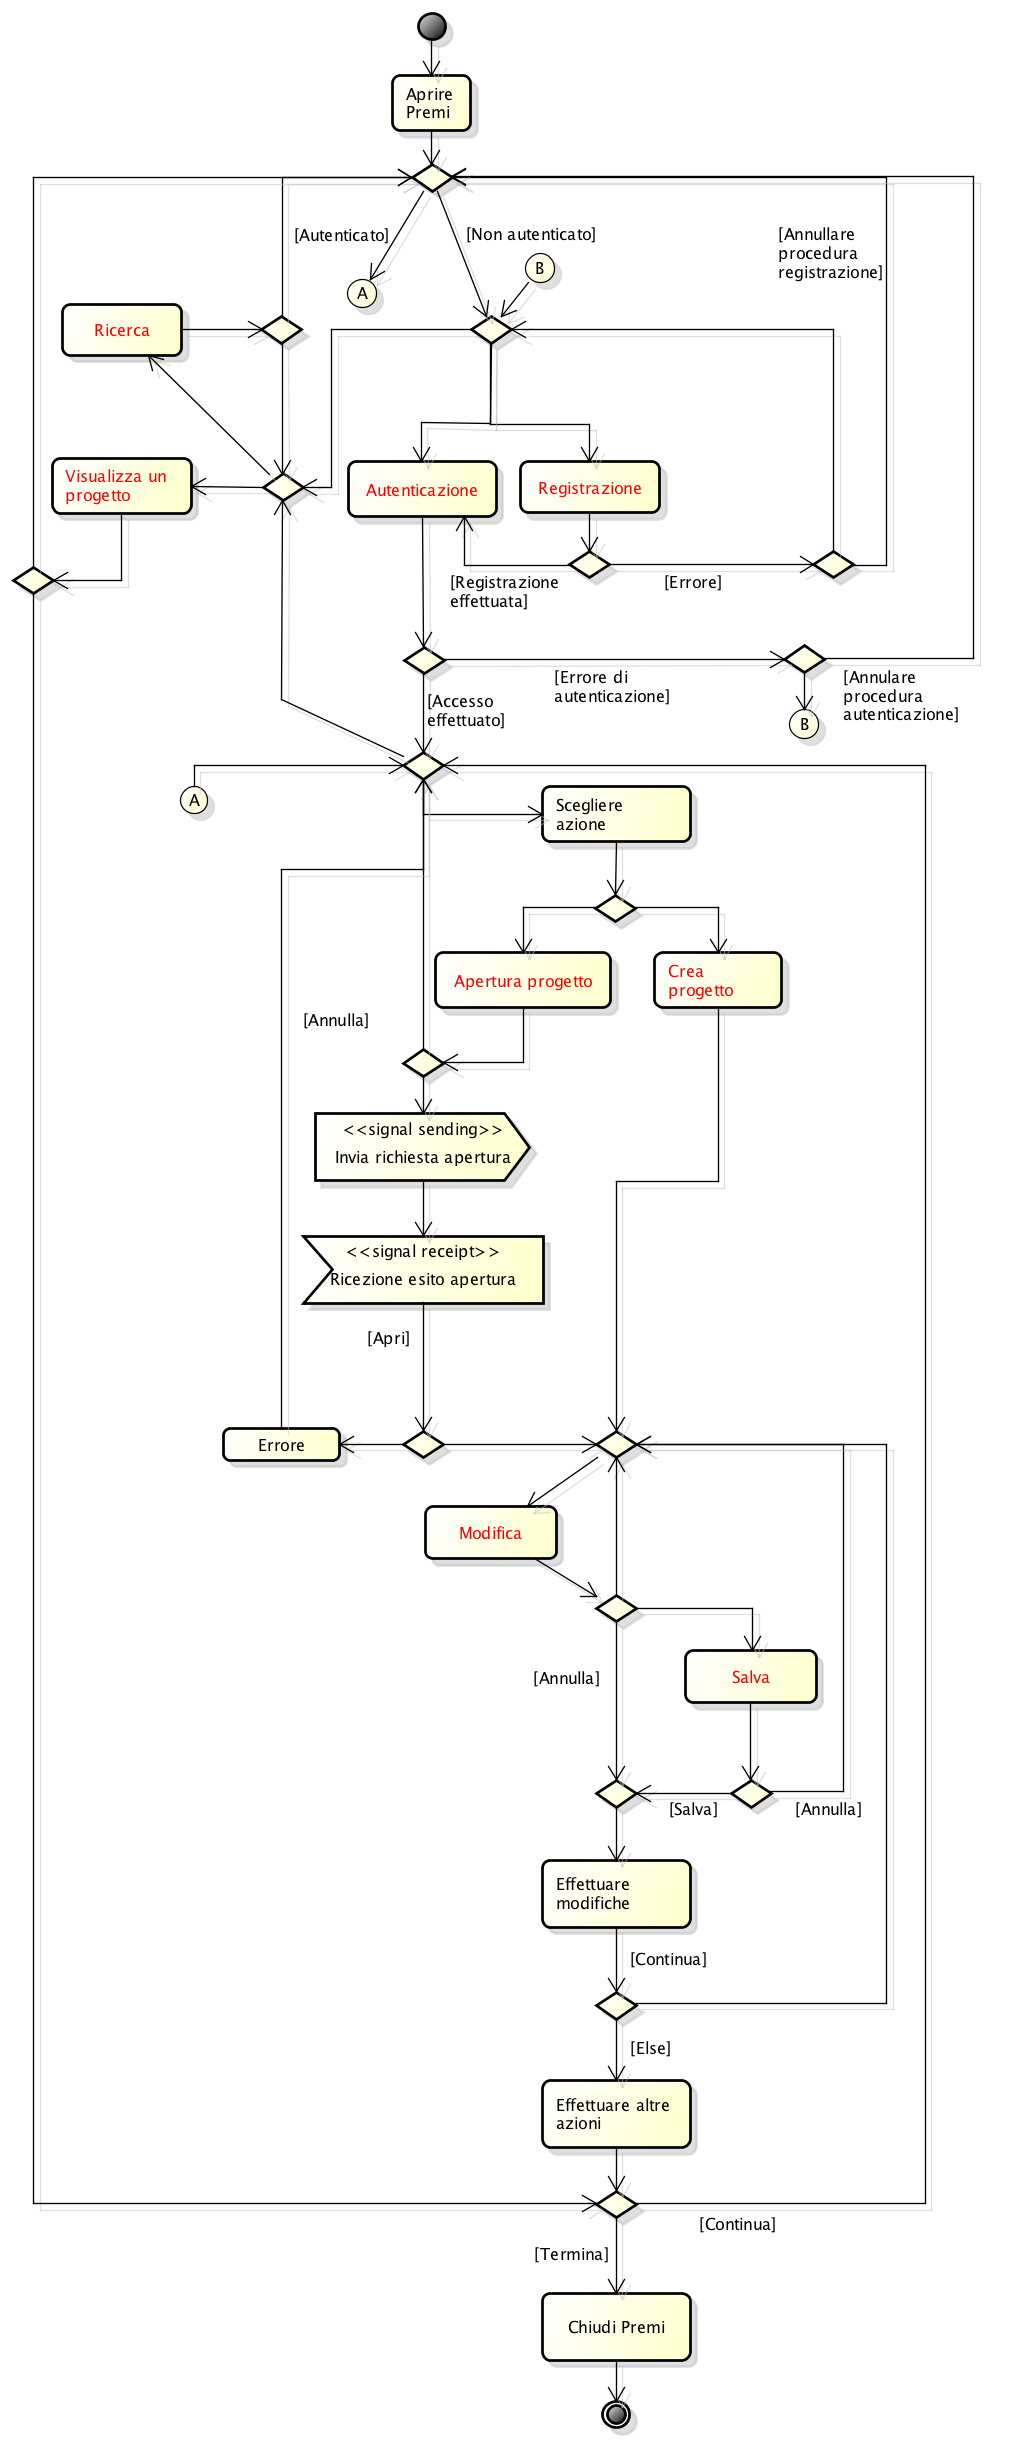
\includegraphics[height=20cm, keepaspectratio] {img/activity_diagram.png}
	\caption{Diagramma attività - Attività principali dell'applicativo \PROGETTO} 
\end{figure}

\newpage

\subsection{Ricerca di un progetto}
\begin{figure}[h] 
	\centering 
	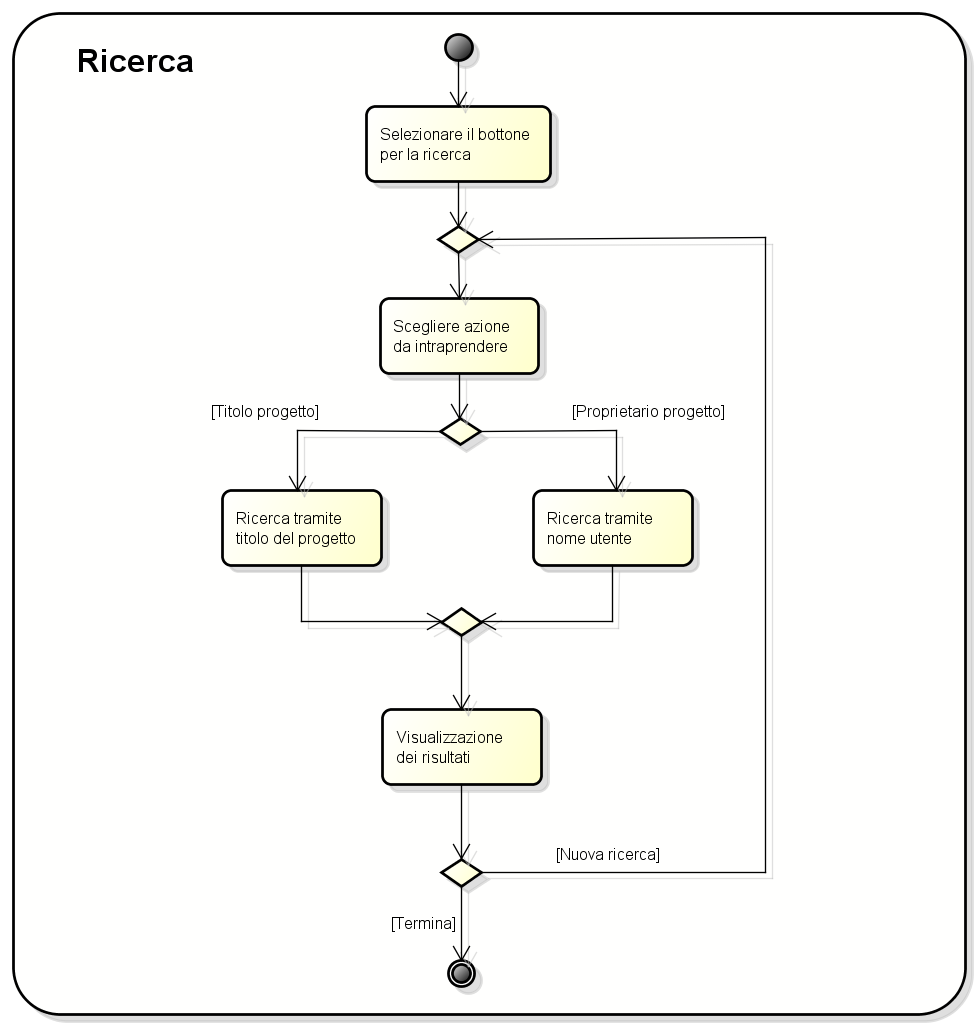
\includegraphics[width=0.9\linewidth] {img/activity_ricerca.png}
	\caption{Diagramma attività - Ricerca di un progetto} 
\end{figure}
Per effettuare una ricerca l'utente deve inserire la chiave di ricerca nell'apposito form e premere il pulsante di ricerca. La chiave di ricerca può essere o il titolo di un progetto o il nome di un utente. Una volta avviata la ricerca, l'utente potrà vedere i risultati e scegliere se effettuare un'altra ricerca o terminare le ricerche.
\newpage

\subsection{Visualizzare un progetto}
\begin{figure}[h] 
	\centering 
	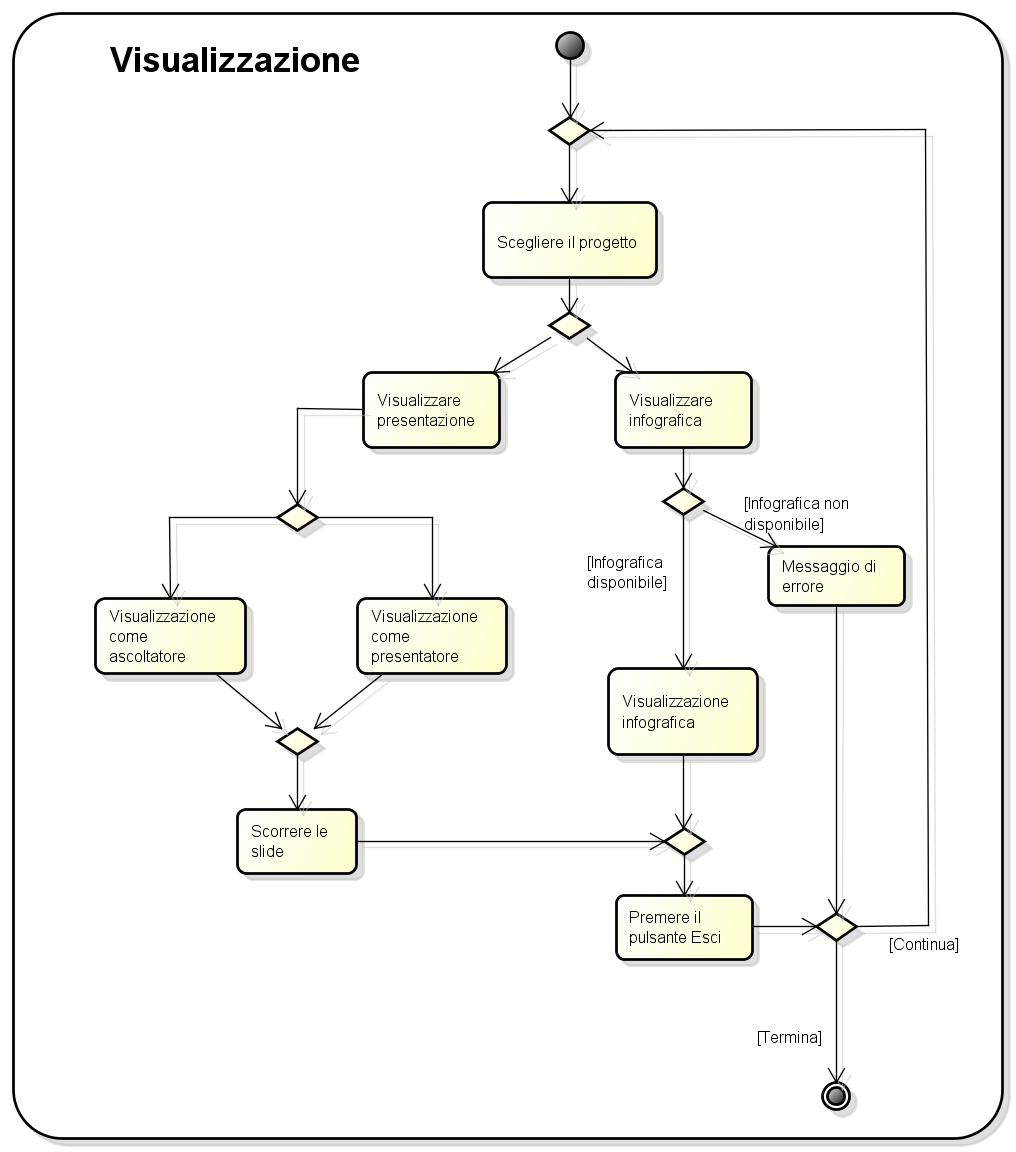
\includegraphics[width=0.9\linewidth] {img/activity_visualizza.png}
	\caption{Diagramma attività - Visualizzare un progetto} 
\end{figure}
Una volta selezionato un progetto permette, l'utente può visualizzare la presentazione oppure l'\gls{infografica} legata al progetto (se essa é disponibile). Nel caso si scelga di visualizzare una presentazione l'utente si può muovere tra le \gls{slide}. Se l'utente vuole uscire dalla presentazione potrà farlo premendo il pulsante esci, e potrà scegliere di visualizzare un'altra presentazione oppure di terminare l'attività di visualizzazione.
\newpage


\subsection{Registrazione}
\begin{figure}[h] 
	\centering 
	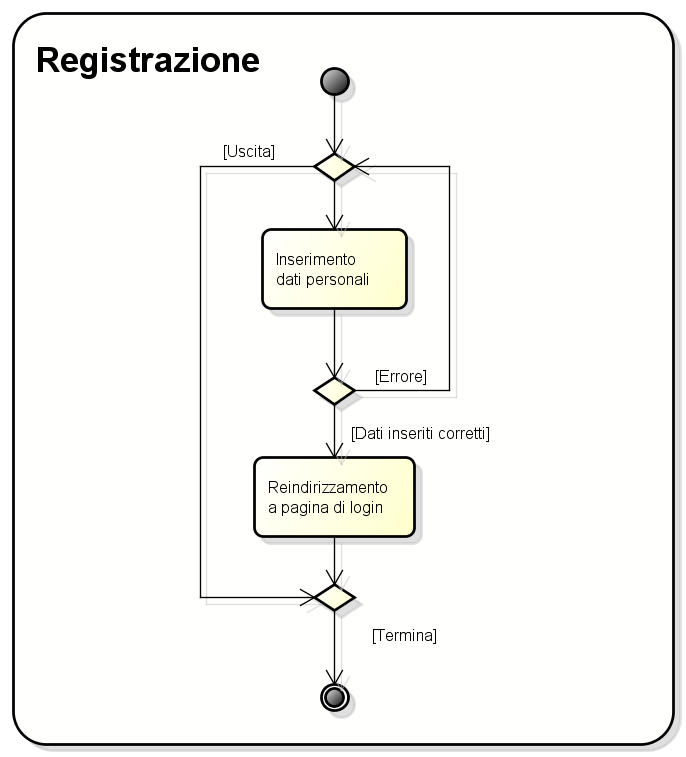
\includegraphics[scale=0.6] {img/activity_registrazione.png}
	\caption{Diagramma attività - Registrazione} 
\end{figure}
La figura rappresenta l'attività di registrazione di un utente. Una volta premuto il pulsante di registrazione, l'utente dovrà inserire i propri dati. Una volta confermati i dati inseriti, se corretti l'utente viene registrato e reindirizzato alla pagina di login, in caso di errore dovrà ripetere la procedura.
\newpage


\subsection{Autenticazione}
\begin{figure}[h] 
	\centering 
	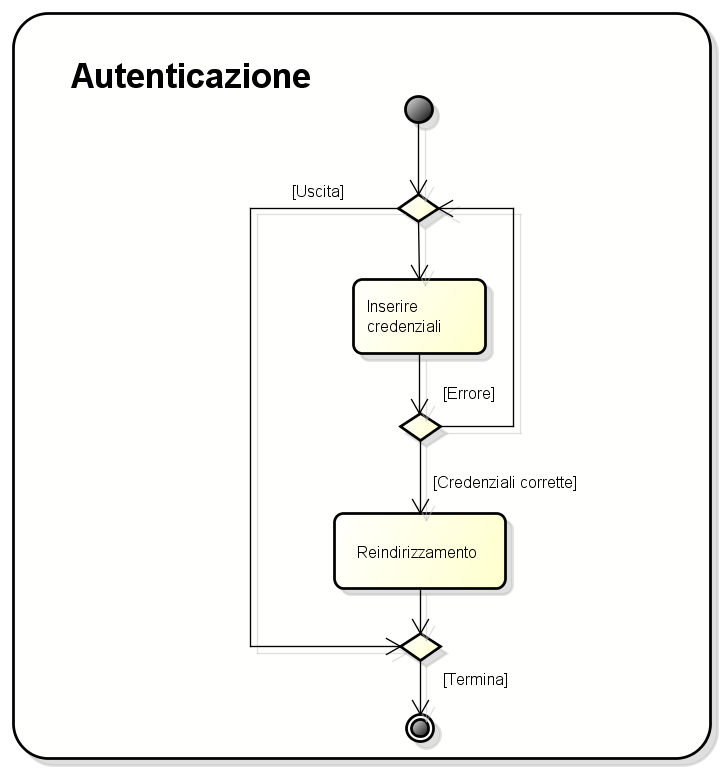
\includegraphics[width=0.9\linewidth] {img/activity_login.png}
	\caption{Diagramma attività - Autenticazione} 
\end{figure}
La figura descrive l'attività di autenticazione di un utente. Una volta premuto il pulsante di login verrà chiesto all'utente di inserire le proprie credenziali e di confermarle. In caso di errore dovrà ripetere la procedura oppure uscire. Se l'autenticazione ha successo l'utente viene reindirizzato alla pagina personale e l'attività di autenticazione termina.
\newpage


\subsection{Creazione di un progetto}
\begin{figure}[h] 
	\centering 
	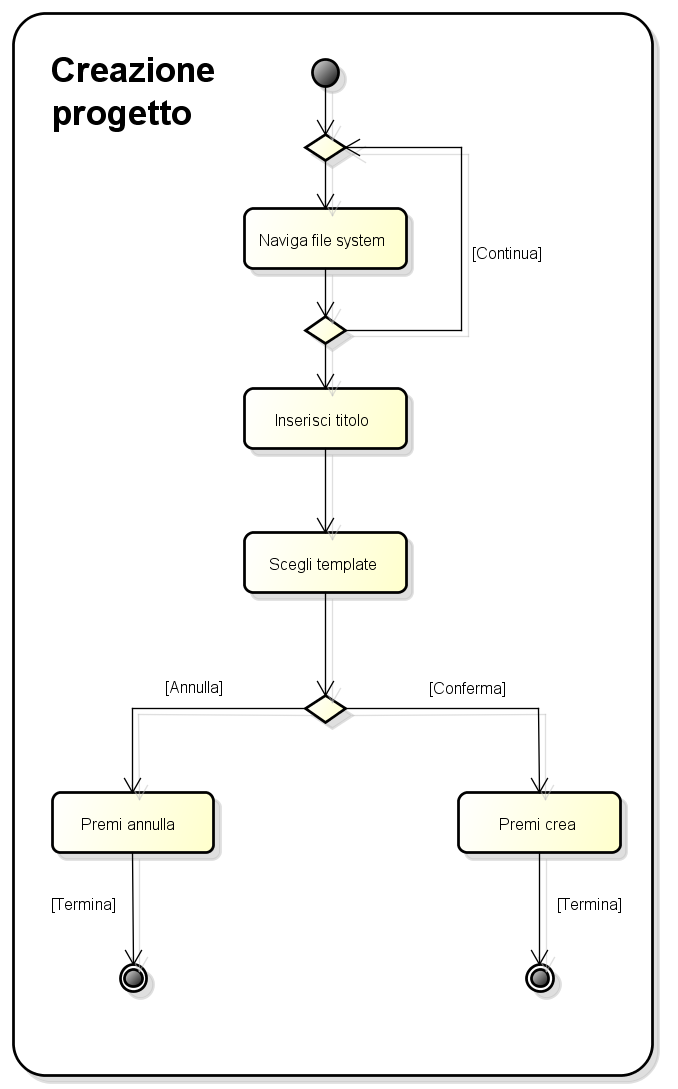
\includegraphics[scale=0.6] {img/activity_creazione.png}
	\caption{Diagramma attività - Creazione di un progetto} 
\end{figure}
Per creare un progetto, all'utente verrà chiesto anzitutto di scegliere un nome per il rpogetto da creare, poi di navigare il file system e scegliere dove salvare il progetto da creare. A questo punto l'utente potrà scegliere se creare il progetto (tramite il pulsante crea), oppure se annullare l'attività di creazione di un progetto.
\newpage


\subsection{Apertura di un progetto}
\begin{figure}[h] 
	\centering 
	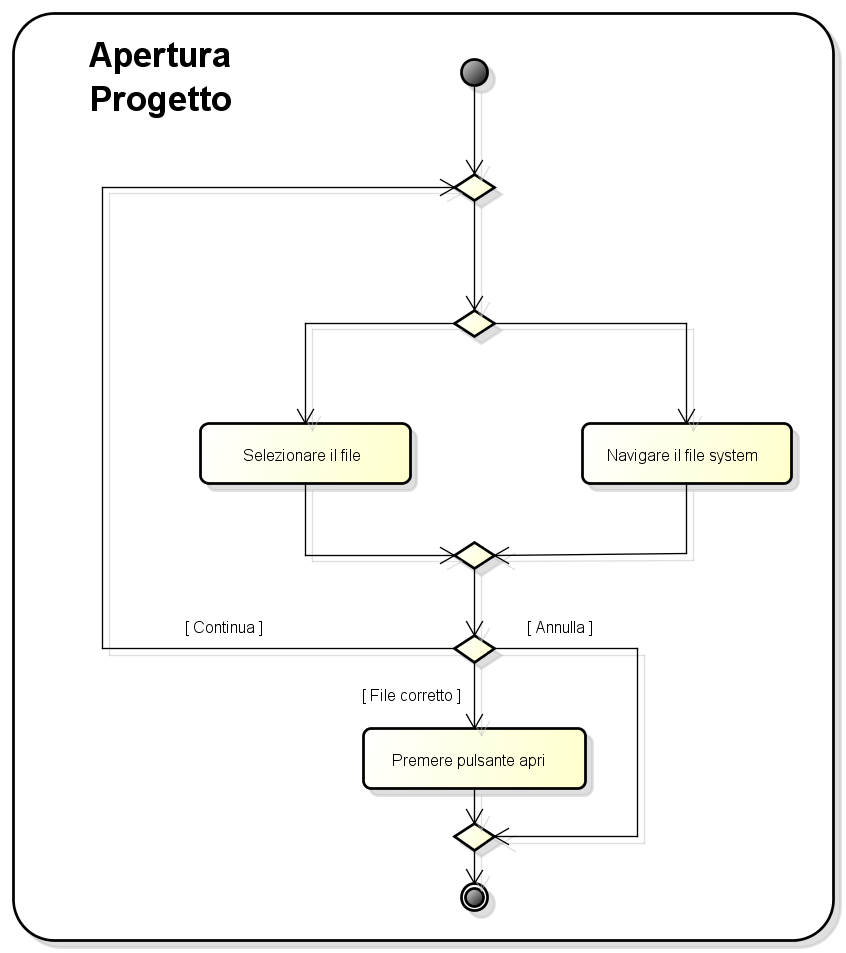
\includegraphics[scale=0.6] {img/activity_apertura.png}
	\caption{Diagramma attività - Apertura di un progetto} 
\end{figure}
Per aprire un progetto precedentemente creato, l'utente deve navigare il file system finché non trova il progetto da aprire e aprirlo tramite il pulsante apri. Oppure può annullare l'apertura. In entrambi i casi l'attività di apertura termina.
\newpage

\subsection{Modifica di un progetto}
\begin{figure}[h] 
	\centering 
	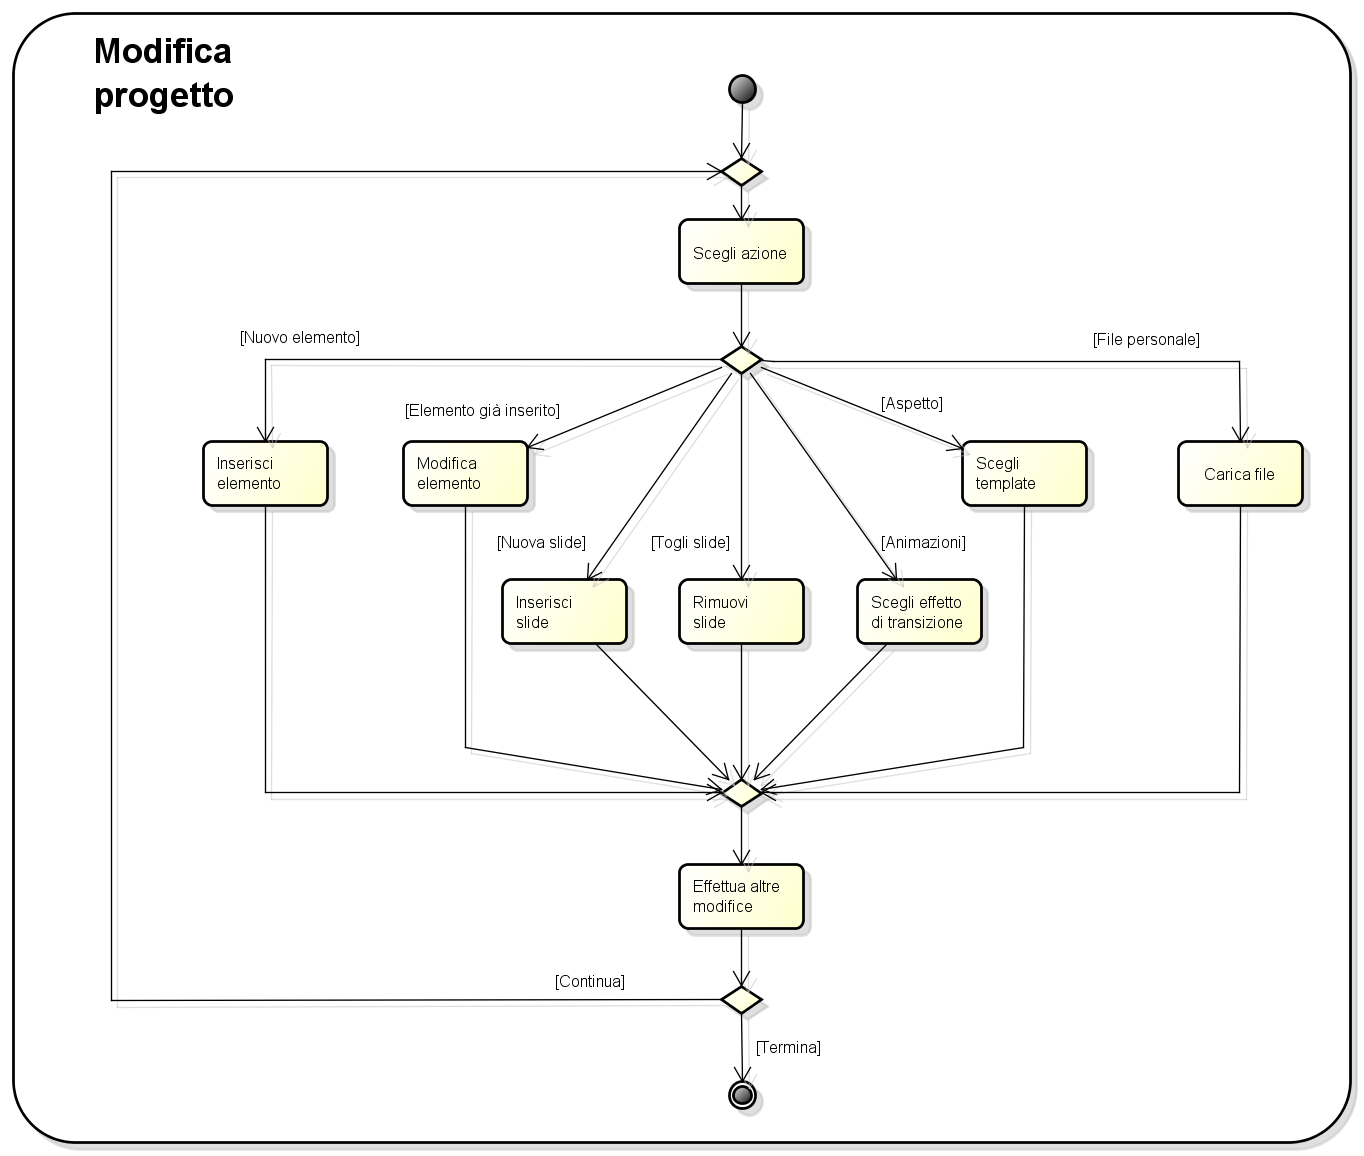
\includegraphics[width=0.9\linewidth] {img/activity_modifica.png}
	\caption{Diagramma attività - Modifica di un progetto} 
\end{figure}
L'attività di modifica permette all'utente di inserire e modificare elementi (come testo, immagini, grafici, ecc...)  nella presentazione corrente tramite la pressione del relativo pulsante. L'utente può inoltre aggiungere e rimuovere \gls{slide}, scegliere un diverso \gls{template} e cambiare l'effetto di transizione tra una \gls{slide} e l'altra. Una volta finito di apportare le modifiche l'attività termina.
\newpage

\subsection{Salvataggio di un progetto}
\begin{figure}[h] 
	\centering 
	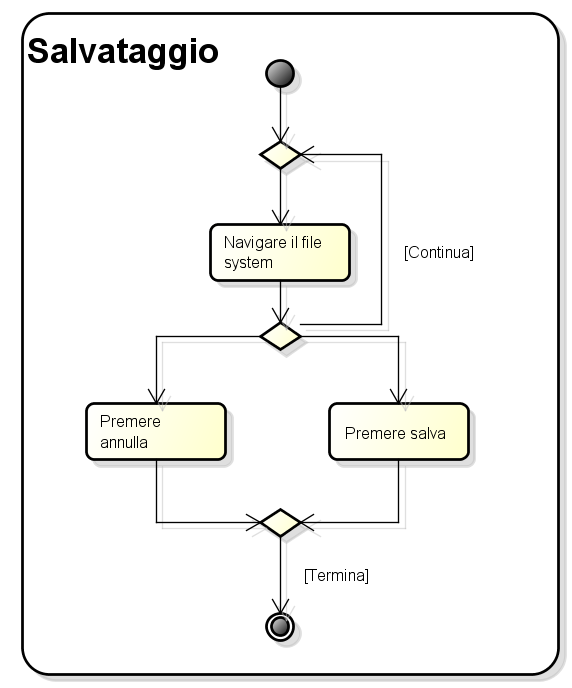
\includegraphics[width=0.6\linewidth] {img/activity_salvataggio.png}
	\caption{Diagramma attività - Salvataggio di un progetto} 
\end{figure}
La figura rappresenta l'attività di salvataggio di un progetto. Lo schema indica la possibilità per l'utente di navigare il file system fino alla posizione desiderata e di salvare oppure annullare il salvataggio. In entrambi i casi alla fine l'attività di salvataggio termina.
\newpage
